
\chapter{Antenna Design Sketches and Parameters}\label{sketch-param}
% 
%
%
\begin{figure}[!htbp]
 \begin{center}
  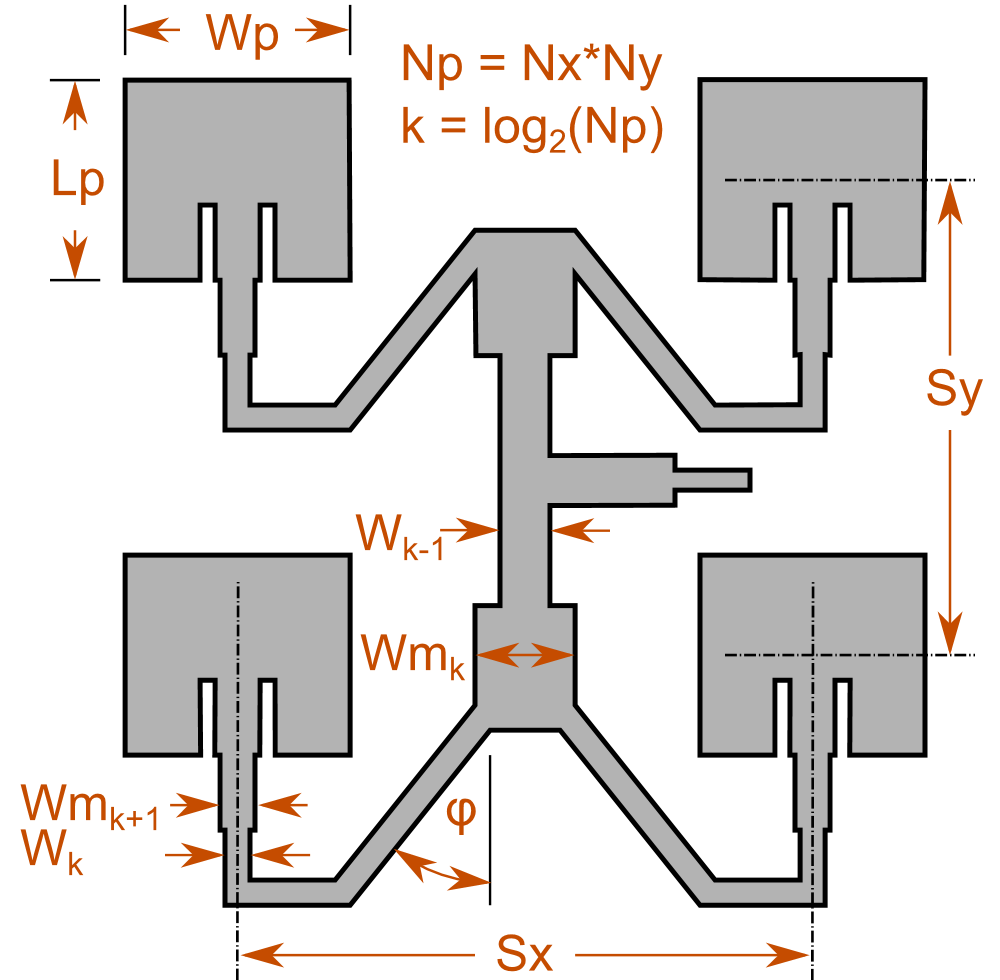
\includegraphics[width=0.5\textwidth]{AM-topview1.png}
 \end{center}
 \caption{Top view of the antenna design. (Source: AntennaMagus software V2017.)}
  \label{fig:tp1}
\end{figure}
% 
%
%



% 
%
%
\begin{figure}[!htbp]
 \begin{center}
  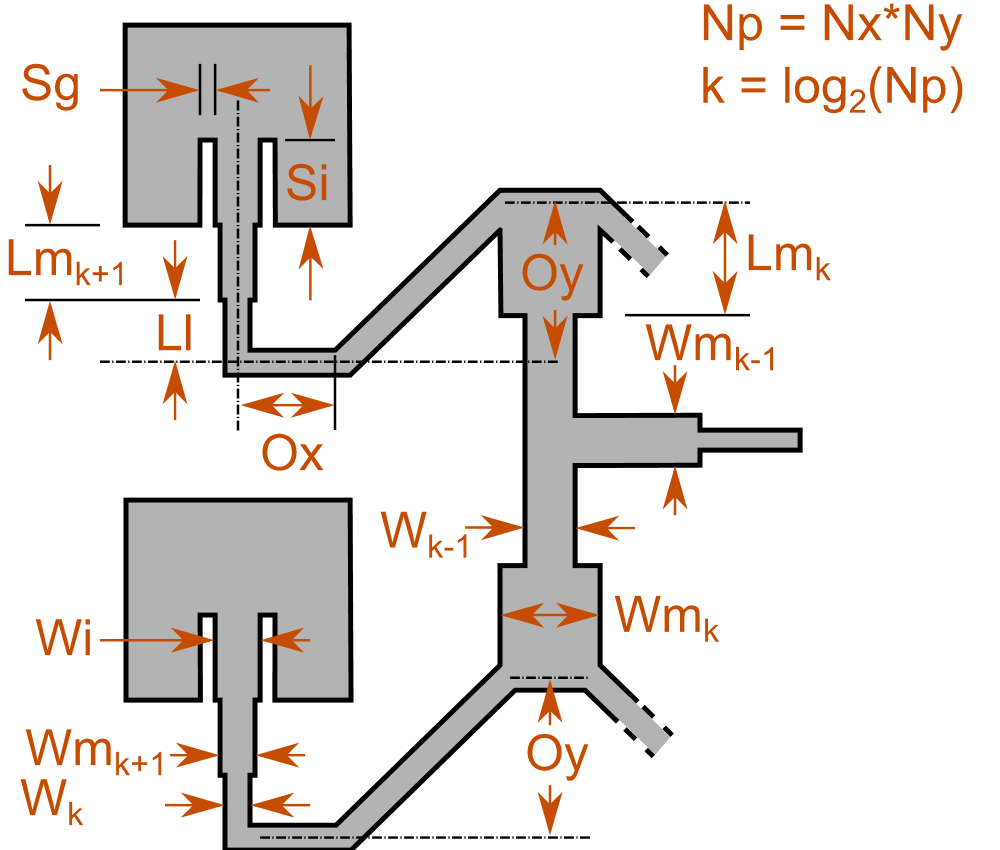
\includegraphics[width=0.5\textwidth]{AM-topview2.png}
 \end{center}
 \caption{Detailed top view of the antenna design. (Source: AntennaMagus software V2017.)}
  \label{fig:tp2}
\end{figure}
% 
%
%



% 
%
%
\begin{figure}[!htbp]
 \begin{center}
  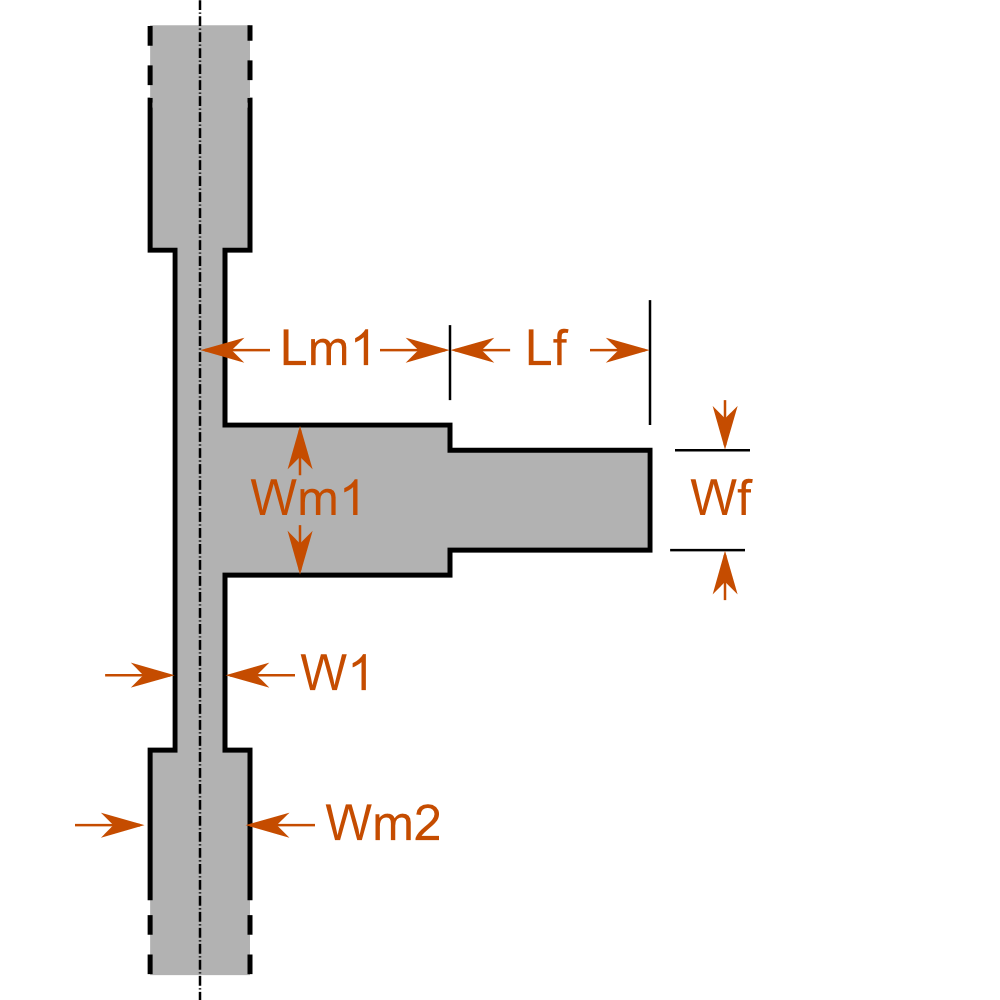
\includegraphics[width=0.5\textwidth]{AM-feed-detail.png}
 \end{center}
 \caption{Feeding network details of the antenna design. (Source: AntennaMagus software V2017.)}
  \label{fig:feed-detail}
\end{figure}
% 
%
%
% 
% Greek letter \textmu{} in normal text.
%   Greek letter µ in normal text.
%   The unit for viscosity is \si{\micro\pascal}.
%   Just the \si{\micro} is not a SI unit but it works anyway.
%   Some number with unit \SI{51}{\micro\metre} lorem ipsum.
%   A number with unit in a formula $\SI{123}{\micro\metre}$ dolor sit amet.
%   
%   
%   \textregistered\textcopyright
% \sffamily\textregistered\textcopyright
% 
% 
% Before: Matlab\textregistered
% 
% After: Matlab\,\textsuperscript{\tiny\textregistered}
% 
% MATLAB\textsuperscript \textregistered / Simulink


% 
%
%
\begin{figure}[!htbp]
 \begin{center}
  
\includegraphics[width=0.5\textwidth]{AM-sideview.png}
 \end{center}
 \caption{Side view details of the antenna design. (Source: AntennaMagus software V2017.)}
  \label{fig:sidev}
\end{figure}
% 
%
%
%
%
%
\renewcommand{\arraystretch}{1.25}%
\begin{table}[H]
\begin{center}
\caption{Antenna parameters and objectives used in the design. (Source: AntennaMagus software V2017.)}
\label{tab:am-params}
\begin{adjustbox}{max width=\textwidth}
\begin{tabular}{| l | l | l | l | l |}
\hline
\rowcolor{lightgray}
\textbf{Type}  &  \textbf{Description}  &  \textbf{ShortName}  &  \textbf{Value}  &  \textbf{Unit}  \tabularnewline
\hline \hline 
Objective  &  Centre frequency  &  f$_{0}$  &  2.4  &  GHz                                             \tabularnewline \hline
Objective  &  Input resistance  &  Rin  &  50  &  \textOmega                                                   \tabularnewline \hline
Objective  &  The substrate name. & Name  &  FR4   & -                                                       \tabularnewline \hline
Objective  &  The substrate manufacturer & Manufacturer  &  Generic    & -                                   \tabularnewline \hline
Objective  &  The thickness of the substrate& Substrate Thickness  &  1.5  &  mm                           \tabularnewline \hline
Objective  &  The relative permittivity of the substrate & Relative Permittivity  &  4.35   & -              \tabularnewline \hline
Parameter  &  Number of patches in X-direction  &  Nx  &  2 patches     & -                                  \tabularnewline \hline
Parameter  &  Number of patches in Y-direction  &  Ny  &  2 patches    & -                                   \tabularnewline \hline
Parameter  &  Patch width  &  Wp  &  37.50  &  mm                                                   \tabularnewline \hline
Parameter  &  Patch length  &  Lp  &  29.09  &  mm                                                  \tabularnewline \hline
Parameter  &  Patch spacing between patch centres in the X-direction  &  Sx  &  87.44 &  mm        \tabularnewline \hline
Parameter  &  Patch spacing between patch centres in the Y-direction  &  Sy  &  87.44  &  mm        \tabularnewline \hline
Parameter  &  X-offset of patch element  &  Ox  &  18.75  &  mm                                     \tabularnewline \hline
Parameter  &  Y-offset of patch element  &  Oy  &  15.65  &  mm                                     \tabularnewline \hline
Parameter  &  Substrate height  &  H  &  1.5  &  mm                                                        \tabularnewline \hline
Parameter  &  Relative permittivity  &  {\textepsilon}r  &  4.35      & -                                      \tabularnewline \hline
Parameter  &  Loss tangent  &  tan{\textdelta}  &  0            & -                                            \tabularnewline \hline
Parameter  &  Matching line 1 length  &  Lm1  &  16.81 &  mm                                       \tabularnewline \hline
Parameter  &  Matching line 2 length  &  Lm2  &  16.81 &  mm                                       \tabularnewline \hline
Parameter  &  Matching line 3 length  &  Lm3  &  8.68  &  mm                                      \tabularnewline \hline
Parameter  &  Matching line 4 length  &  Lm4  &  18.05 &  mm                                       \tabularnewline \hline
Parameter  &  Matching line 5 length  &  Lm5  &  18.05  &  mm                                       \tabularnewline \hline
Parameter  &  Matching line 6 length  &  Lm6  &  18.05  &  mm                                       \tabularnewline \hline
Parameter  &  Matching line 7 length  &  Lm7  &  18.05  &  mm                                       \tabularnewline \hline
Parameter  &  Matching line 1 width  &  Wm1  &  4.933  &  mm                                       \tabularnewline \hline
Parameter  &  Matching line 2 width  &  Wm2  &  4.933  &  mm                                       \tabularnewline \hline
Parameter  &  Matching line 3 width  &  Wm3  &  2.892  &  mm                                       \tabularnewline \hline
Parameter  &  Matching line 4 width  &  Wm4  &  673.9   &  \SI{}{\um}                                     \tabularnewline \hline
Parameter  &  Matching line 5 width  &  Wm5  &  673.9   &  \SI{}{\um}                                       \tabularnewline \hline
Parameter  &  Matching line 6 width  &  Wm6  &  673.9   &  \SI{}{\um}                                       \tabularnewline \hline
Parameter  &  Matching line 7 width  &  Wm7  &  673.9   &  \SI{}{\um}                                       \tabularnewline \hline
Parameter  &  Network line 1 width  &  W1  &  2.892  &  mm                                         \tabularnewline \hline
Parameter  &  Network line 2 width  &  W2  &  2.892  &  mm                                         \tabularnewline \hline
Parameter  &  Network line 3 width  &  W3  &  673.9   &  \SI{}{\um}                                           \tabularnewline \hline
Parameter  &  Network line 4 width  &  W4  &  673.9   &  \SI{}{\um}                                         \tabularnewline \hline
Parameter  &  Network line 5 width  &  W5  &  673.9   &  \SI{}{\um}                                         \tabularnewline \hline
Parameter  &  Network line 6 width  &  W6  &  673.9   &  \SI{}{\um}                                        \tabularnewline \hline
Parameter  &  Network line length  &  Ll  &  4.339  &  mm                                          \tabularnewline \hline
Parameter  &  Feed line length  &  Lf  &  4.339  &  mm                                             \tabularnewline \hline
Parameter  &  Feed line width  &  Wf  &  2.892  &  mm                                              \tabularnewline \hline
Parameter  &  Feed inset from edge of patch  &  Si  &  10.53  & mm                                 \tabularnewline \hline
Parameter  &  Width of patch feed line  &  Wi      &  2.892  &  mm                                  \tabularnewline \hline
Parameter  &  Spacing between feed line and patch  &  Sg  &  2.892  &  mm                           \tabularnewline \hline
Derived  &  Device X-dimension  &  X  &  124.9  &  mm                                                  \tabularnewline \hline
Derived  &  Device Y-dimension  &  Y  &  131.0  &  mm                                                \tabularnewline \hline
Derived  &  Device Z-dimension  &  Z  &  1.5  &  mm                                                        \tabularnewline \hline
Derived  &  Angle of diagonal lines  &  \textphi  &  56.36 & \textdegree                         \tabularnewline \hline
\end{tabular}
%\\[1.0] %You can adjust how far below the table the text should appear
\end{adjustbox}
\end{center}
\end{table}
\renewcommand{\arraystretch}{1}%      






                                                                                                            
